\documentclass{report}

\usepackage{amsmath,amsfonts}
\usepackage{authblk}
\usepackage{graphicx}
\usepackage{caption,subcaption}
%\usepackage{color}
%\usepackage{etoolbox}
\usepackage{float}
\usepackage{fullpage}
%\usepackage{mathtools}
\usepackage{natbib}
\usepackage{paralist}
%\usepackage{setspace}

\renewcommand\thesection{\arabic{section}}
\usepackage{xspace}
\newcommand{\textcompute}{\textsf}
\newcommand{\N}{\text{N}} % Normal 
\newcommand{\R}{\textcompute{R}\xspace}
\newcommand{\IG}{\text{InvGam}}
\newcommand{\RL}{f}
\newcommand{\RLorig}{\text{RL}}
\newcommand{\logRL}{\log\RL}
\newcommand{\logRLorig}{\log\RLorig}
\newcommand{\sigssq}{\sigma_s^2}
\newcommand{\sigesq}{\sigma_e^2}
\newcommand{\sshat}{\hat\sigma^2_e,\hat\sigma^2_s}
\newcommand{\logRLss}{\logRL(\sigesq,\sigssq)}
\newcommand{\logRLssorig}{\logRLorig(\sigesq,\sigssq)}
\newcommand{\ass}{a_j\sigssq + \sigesq}
\newcommand{\abss}{a_j\sigssq + b_j\sigesq}
\newcommand{\fss}{f(\sigesq,\sigssq)\,}
%\newcommand{\mrle}{MRLE}
\newcommand{\mrle}{$\argsup\log f$}
%\newcommand{\lone}{\textbf{l}_1}
%\newcommand{\pone}{\textbf{p}_1}
%\newcommand{\ltwo}{\textbf{l}_2}
%\newcommand{\ptwo}{\textbf{p}_2}
%\newcommand{\pthree}{\textbf{p}_3}
%\newcommand{\given}{\,|\,}
\newcommand{\g}{\,|\,}
\newcommand{\maxit}{\textcompute{maxit}}
\newcommand{\argmax}{\operatornamewithlimits{argmax}}
\newcommand{\argsup}{\operatornamewithlimits{argsup}}
\renewcommand{\bibname}{References}


\begin{document}

\title{Approximately Exact Calculations for Linear Mixed Models}
%\author[1]{Michael Lavine}
%\author[2]{James Hodges}
%\affil[1]{Department of Mathematics and Statistics, University of Massachusetts, Amherst, MA 01003 USA}
%\affil[2]{Division of Biostatistics, University of Minnesota, Minneapolis, MN 55455 USA}
 %for blinding
\author[1]{Arlene A. Author}
\author[2]{Sheldon Scrivener}
\affil[1]{University of Whales}
\affil[2]{School of Fish}

\maketitle

\begin{abstract}
This paper is about computations for linear mixed models having two variances, $\sigma^2_e$ for residuals and $\sigma^2_s$ for random effects, though the ideas can be extended to some linear mixed models having more variances.  Researchers are often interested in either the restricted (residual) likelihood $\RLorig(\sigesq,\sigssq)$ or the joint posterior $\pi(\sigesq,\sigssq\g y)$ or their logarithms.  Both $\log\RLorig$ and $\log\pi$ can be multimodal and computations often rely on either a general purpose optimization algorithm or MCMC, both of which can fail to find regions where the target function is high.  This paper presents an alternative.  Letting $f$ stand for either $\RLorig$ or $\pi$, we show how to find a box $B$ in the $(\sigesq,\sigssq)$ plane such that
\begin{enumerate}
\item all local and global maxima of $\log f$ lie within $B$;
\item $\sup_{(\sigesq,\sigssq) \in B^c} \log f(\sigesq,\sigssq) \le \sup_{(\sigesq,\sigssq) \in B} \log f(\sigesq,\sigssq) - M$ for a prespecified $M>0$; and
\item $\log f$ can be estimated to within a prespecified tolerance $\epsilon$ everywhere in $B$ with no danger of missing regions where $\log f$ is large.
\end{enumerate}
Taken together these conditions imply that the $(\sigesq,\sigssq)$ plane can be divided into two parts: $B$, where we know $\log f$ as accurately as we wish,  and $B^c$, where $\log f$ is small enough to be safely ignored.  We provide algorithms to find $B$ and to evaluate $\log f$ as accurately as desired everywhere in $B$.
\end{abstract}

\section{Introduction}
\label{sec:intro}
Linear mixed models are an important class of statistical models.  Books are written about them (e.g.\ \citealt{bryk_raudenbush:1992, verbeke&molenberghs:2000, hodges:2013, west&welch&galecki:2014}),  courses are taught about them, and they have many applications.  Examples include random intercept models (including balanced and unbalanced one-way random effect models), additive models with one penalized spline, spatial models with one intrinsic conditional autoregression (ICAR) random effect, dynamic linear models with one system-level variance, and some multiple membership models (e.g.\ \citealt{browne_etal:2001, mccaffrey_etal:2004}).  Typical notation, which we adopt, is
\begin{equation}
\label{eq:lmm}
	y = X\beta + Zu + \epsilon
\end{equation}
where $y$ is a vector of $n$ observations, $X$ is a known $n \times p$ matrix, $\beta$ is a vector of $p$ unknown coefficients called fixed effects, $Z$ is a known $n \times q$ matrix, $u$ is a vector of $q$ unknown coefficients called random effects, and $\epsilon$ is a vector of $n$ errors. The term ``mixed" is used when we treat $u$ as a vector of random variables, thus mixing fixed and random effects in the same model.  For linear mixed models where $u$ and $\epsilon$ are modelled as Normal, researchers are often interested in the restricted likelihood function
\begin{equation}
\label{eq:rll}
  \RLorig(\theta) = K |V(\theta)|^{-1/2}|X^tV^{-1}(\theta)X|^{-1/2}
                       \exp\left\{ -\frac{1}{2} \left(y^tV^{-1}(\theta)y -
                                                                \tilde\beta^t(\theta)X^tV^{-1}(\theta)X\tilde\beta(\theta)
                                                         \right)
                              \right\}
\end{equation}
where $K$ is an unimportant constant, $\theta$ is a vector of unknown parameters in the covariance matrices of $u$ and $\epsilon$, $V(\theta)$ is the marginal covariance matrix of $y$ implied by the covariance matrices of $u$ and $\epsilon$, and $\tilde\beta(\theta)$ is the generalized least-squares estimate of $\beta$, given $V(\theta)$.
This manuscript deals with the special case in which we adopt the model
\begin{equation*}
	\epsilon \sim \N (0, \sigma_e^2 \Sigma_e) \qquad u \sim \N (0, \sigma_s^2 \Sigma_s)
\end{equation*}
where $\Sigma_e$ and $\Sigma_s$ are known matrices, often the identity, of the appropriate sizes and $\theta \equiv (\sigma_e^2, \sigma_s^2)$, two unknown variance parameters.  The key for this manuscript is that $\theta$ contains only those two unknown variances and no others.  \cite{hodges:2013} gives examples and explains the importance of this special case.

\cite{hodges:2013} also unifies and generalizes \cite{reich_hodges:2008} and \cite{welham_thompson:2009} to show that in our special case, and a few others, $\logRLssorig$ can be expressed as
\begin{equation}
\label{eq:reexpress}
  \logRLssorig = B - \frac{n_e}{2}\log(\sigesq) - \frac{y^t \Gamma_c \Gamma^t_c y}{2\sigesq} 
    - \frac{1}{2} \sum_{j=1}^{s_z} \left[ \log(\ass) + \frac{\hat v_j^2}{\ass}\right]
\end{equation}
where $B$ is an unimportant known constant; $n_e$ is $n$ minus the dimension of the space spanned by the columns of $[X|Z]$; $\Gamma_c$ is $n \times n_e$ and spans the space orthogonal to $[X|Z]$ (so $y^t \Gamma_c \Gamma^t_c y$ is the residual sum of squares); $s_z$ is the dimension of the space spanned by the columns of $Z$ not already in the span of the columns of $X$; and the $\{a_j\}$ and $\{\hat v_j\}$ are known constants with all $a_j>0$.  Thus the only unknowns are $(\sigma^2_s, \sigma^2_e)$ and $\logRLssorig$ is a function of just those two arguments.  Specifically, $\logRLssorig$ is a linear combination of logs and inverses of linear functions $\abss$ of the two unknowns.

As \cite{hodges:2013} further observes, if $\beta$ is given an improper flat prior and $\sigesq$ and $\sigssq$ are given conjugate priors --- say $\sigesq \sim \IG(\alpha_e,\beta_e)$ and $\sigssq \sim \IG(\alpha_s,\beta_s)$ --- then \begin{equation*}
  -(\alpha_e+1) \log\sigesq - \beta_e/\sigesq -(\alpha_s+1) \log\sigssq - \beta_s/\sigssq
\end{equation*}
is added to \eqref{eq:reexpress} to yield
the log posterior
\begin{equation}
\label{eq:logpost}
  \begin{split}
  \log\pi(\sigesq,\sigssq\g y) &=
  B - \frac{n_e + 2\alpha_e + 2}{2}\log(\sigesq) -
    \frac{y^t \Gamma_c \Gamma^t_c y + 2\beta_e}{2\sigesq}\\
    &\qquad\qquad - \frac{2\alpha_s + 2} {2}\log(\sigssq) - \frac{2\beta_s}{2\sigssq}
    - \frac{1}{2} \sum_{j=1}^{s_z} \left[ \log(\ass) + \frac{\hat v_j^2}{\ass}\right]\\
    &= B - \frac{1}{2}\sum_j\left[ c_j \log(\abss) + \frac{d_j}{\abss}\right]
  \end{split}
\end{equation}
for known nonnegative constants $\{a_j, b_j, c_j, d_j\}$ ---
still a linear combination of logs and inverses of linear functions $\abss$.  Our derivation will proceed from \eqref{eq:logpost}, though it applies also to \eqref{eq:reexpress} and other linear combinations of logs and inverses of linear functions $\abss$.  We use $f$ to denote such functions generically.  

It is known (e.g.\ \citealt{henn&hodges:2014}) that $\logRLss$\  
can have multiple maxima and that existing general purpose algorithms for linear mixed models may fail to find all of them, as shown by examples in \cite{hodges:2013}, \cite{henn&hodges:2014}, and elsewhere.
\cite{mullen:2014} examines 18 optimization functions available in \R, tests them on 48 objective functions (admittedly more complicated than $\logRLss$) and finds that even the best of them fail in over 10\% of the cases.  \cite{henn&hodges:2014} examine conditions under which multiple maxima occur in posterior densities and conclude ``\dots second maxima in posterior distributions therefore may be more common than reports in the literature would suggest."  Thus, failure to find local and global maxima may be common.  

Our point of view is that it is important to find regions where $f$ or $\log f$ is large relative to its maximum regardless of whether the regions contain local maxima.  (E.g., if $f$ or $\log f$ is relatively flat and large over a region, it matters little whether the region contains small bumps that are, technically, local maxima.)  This paper shows how to find $(\sshat) \equiv \argsup_{\sigesq, \sigssq}\logRLss$ globally (typically either the maximum restricted log likelihood estimate or the maximum \textit{a posteriori} estimate) and to evaluate $\logRLss$ everywhere, each to within a prespecified tolerance (hence ``approximately exact''), without fear of missing regions of high $f$ or $\logRL$.  The technique relies on the partial derivatives of $\logRLss$.  Analysis of the partial derivatives allows us to satisfy two desiderata.
\begin{description}
\item[D1] For any prespecified constant $M>0$ we can find a box $B$, a rectangle in the first quadrant of the $(\sigssq, \sigesq)$ plane whose sides are parallel to the axes, such that
\begin{equation}
\label{eq:boundingbox}
	\text{all local maxima are in $B$} \qquad \text{and} \qquad \sup_{(\sigesq, \sigssq) \in B^c} \logRLss \le \logRL(\sshat) - M.
\end{equation}
In practice we will take $M$ to be large enough to interpret (\ref{eq:boundingbox}) as meaning that we can restrict attention to $B$ because values of $(\sigesq, \sigssq) \in B^c$ have $\logRLss$ too low to be of further interest.

\item[D2] For any box $b$ we can quickly compute lower and upper bounds $(L^b,U^b)$ satisfying
\begin{equation*}
  L^b \le \inf_{(\sigesq, \sigssq) \in b}\logRLss \qquad\text{and}\qquad
  U^b \ge \sup_{(\sigesq, \sigssq) \in b}\logRLss
\end{equation*}
and such that $U^b-L^b \rightarrow 0$ as $b$ shrinks.  Therefore, partitioning the box $B$ from \textbf{D1} allows us to know $\logRLss$ everywhere in $B$ to within a pre-specified tolerance and also to locate $\argsup\logRL$ to within a pre-specified tolerance without fear of missing regions of high $\logRL$.
\end{description}
The next section shows how the partial derivatives are used to satisfy \textbf{D1} and \textbf{D2}.

\section{Satisfying the Desiderata}
\subsection{Partial Derivatives Determine Lines}
The partial derivatives of $\logRLss$ can be calculated from (\ref{eq:logpost}):
\begin{subequations}
\label{eq:partials}
\begin{equation}
\label{eq:drlds}
  \frac{\partial\logRLss}{\partial\sigssq}
  = -\frac{1}{2} \sum_j
        \left[ \frac{a_jc_j}{\abss} - \frac{a_j d_j}{(\abss)^2} \right]
        = -\frac{1}{2} \sum_j
           \frac{a_j \left( a_jc_j\sigssq + b_jc_j\sigesq  - d_j\right)}{(\abss)^2}\\
\end{equation}
and
\begin{equation}\label{eq:drlde}
  \frac{\partial\logRLss}{\partial\sigesq} =
    -\frac{1}{2} \sum_j \left[ \frac{b_jc_j}{\abss} - \frac{b_j d_j}{(\abss)^2} \right]
    = - \frac{1}{2} \sum_j \frac{b_j \left( a_jc_j\sigssq + b_jc_j\sigesq  - d_j\right)}{(\abss)^2}.
\end{equation}
\end{subequations}
We work with one term in (\ref{eq:partials})'s summations at a time; that is, one $j$ at a time.  The $j$'th terms in (\ref{eq:partials}) differ only by a multiplicative constant $a_j/b_j$; they have the same sign as each other and the same sign as $(a_jc_j\sigssq + b_jc_j\sigesq  - d_j)$, which determines a line $\sigssq = d_j/a_j c_j - b_j \sigesq/a_j$ --- call it the $j$'th line --- in the first quadrant of the $(\sigssq,\sigesq)$ plane.  The line has positive intercept and negative slope because all the constants are nonnegative.  Both partial derivatives of the $j$'th term are positive below the $j$'th line, 0 on the line, and negative above the line, as indicated in Figure~\ref{fig:oneline}.  The $j$'th term is constant on the $j$'th line and attains its maximum there.  Both \eqref{eq:reexpress} and \eqref{eq:logpost} contain a term, call it the $v$'th (for vertical) term,  with $a_j=0$.  The corresponding line is vertical at $\sigesq = \sigma_e^{2v} \equiv d_v / b_v c_v$.  The $v$'th term in (\ref{eq:partials}) is negative to the right of the $v$'th line, positive to the left, and 0 on the line; hence the $v$'th term in \eqref{eq:logpost} is maximized on the $v$'th line.  \eqref{eq:logpost} also contains a term, call it the $h$'th (for horizontal) term, with $b_j=0$.  The corresponding line is horizontal at $\sigssq = \sigma_e^{2h} \equiv d_h / a_h c_h$.  The $h$'th term in \eqref{eq:logpost} is maximized on the $h$'th line.

\begin{figure}[h]
	\centering
	\includegraphics[width=.5\linewidth]{figs/oneline.pdf}
	\caption{For a single summand, i.e., a fixed $j$, in (\ref{eq:logpost}),
	              the partial derivatives (\ref{eq:drlds}) and (\ref{eq:drlde})
	              are 0 on the line and positive and negative where indicated
	              by ``\textbf{+}" and ``\textbf{-}".}
	\label{fig:oneline}
\end{figure}

\subsection{Lines Determine a Bounding Box}
\label{sec:boundingbox}

Figure~(\ref{fig:bigboundingbox}) shows five lines --- realistic data sets may have more --- labelled $j=1, 2, 3, v, h$.  The largest intercept of those lines on the $\sigssq$ axis and the largest intercept on the $\sigesq$ axis determine a rectangle $B_1$ whose outline is marked in bold.  At any point above $B_1$, e.g., $p_1$, the partial derivatives \eqref{eq:partials}, for all $j$, are negative or, for $j=v$, zero.  Therefore, $\logRL(p_1^*) \ge \logRL(p_1)$.  Similarly, for points like $p_2$, $\logRL(p_2) \ge \logRL(p_2^*)$ and, for points like $p_3$, $\logRL(p_3^*) \ge \logRL(p_3)$.  That is, for points above and/or to the right of $B_1$, $\logRLss$ can be increased by moving down and/or to the left as far as $B_1$'s boundary.  Therefore \mrle\ must lie on or inside $B_1$ and there can be no maxima of $\logRLss$ in $B_1^c$.  $B_1$ could be passed to an optimizer such as \R's \textsf{optim} or \textsf{nlminb}, with potentially better results than using those functions without bounds.  However, even with known bounds, general purpose optimizers may still miss \mrle\ and regions of high $\logRL$.  This paper presents a computational method guaranteed not to miss \mrle\ and which evaluates $\logRLss$ everywhere to within a specified tolerance inside a box $B$ satisfying desideratum \textbf{D1}.  First, though, we pause to note that the region outlined in bold in Figure~(\ref{fig:smallboundingbox}) is a subset of $B_1$ that must also contain \mrle\ for the reasons given above.  But it is not rectangular, hence less convenient than $B_1$, so we don't pursue it further.

\begin{figure}[h]
  \begin{subfigure}{.5\textwidth}
	\centering
	\includegraphics[width=.8\linewidth]{figs/boundingbox.pdf}
	\caption{A rectangular region containing all maxima.}
	\label{fig:bigboundingbox}
  \end{subfigure}
  \begin{subfigure}{.5\textwidth}
	\centering
	\includegraphics[width=.8\linewidth]{figs/smallboundingregion.pdf}
	\caption{A smaller region containing all maxima.}
	\label{fig:smallboundingbox}
  \end{subfigure}
  \caption{all local and global maxima lie in the regions bounded by the solid
                dark line.
               }
  \label{fig:boundingbox}
\end{figure}

To find $B$, choose an arbitrary constant $M>0$ and an arbitrary point inside $B_1$, say $p_4$, as illustrated in Figure~(\ref{fig:boundingbox2}) and define $L \equiv \logRL(p_4)$.  We will find a box $B\supset B_1$, as shown in Figure~(\ref{fig:boundingbox2}), outside of which $\logRLss \le L-M$, thus satisfying \textbf{D1}.  We have drawn a figure without an $h$ line so the reader can see  the derivation without it, which would apply to $\logRLorig$.  If there were an $h$ line, it would influence the derivation for Figure~(\ref{fig:boundingbox2})'s $q_1$ in a manner analogous to how the $v$ line influences the argument for $q_2$ and $q_3$.

$B$ is determined by its intercepts $\sigma_e^{2*}$ and $\sigma_s^{2*}$ on the $\sigesq$ and $\sigssq$ axes respectively.  Let $q_1^* = (\sigma_e^{2*},0)$ be the intercept of $B$ and the $\sigesq$ axis.  Because each term of the partial derivatives \eqref{eq:partials} is nonpositive to the right of $B_1$, for any point $q_1$ to the right of $B$, every term in the summation of \eqref{eq:logpost} (with the possible exception of an $h$ term) is larger at $q_1^*$ than at $q_1$.  Therefore, $\logRL(\sshat) - \logRL(q_1) \ge L - \logRL(q_1^*)$.  The latter expression is greater than $M$ iff $\logRL(q_1^*) < L-M$.  But examination of (\ref{eq:logpost}) shows that for any fixed $\sigssq$, in particular for $\sigssq=0$, $\lim_{\sigesq \rightarrow \infty} \logRLss = -\infty$.  Thus by choosing $\sigma_e^{2*}$ large enough so $\logRL(q_1^*) < L-M$, we satisfy (\ref{eq:boundingbox}) for all points with $\sigesq \ge \sigma_e^{2*}$.

Let $q_2^* = (\sigma_e^{2v},\sigma_s^{2*})$.  For any point $q_2$ having $\sigssq \ge \sigma_s^{2*}$ and $\sigesq \in [\sigma_e^{2v}, \sigma_e^{2*}]$ --- i.e., above $B$ and to the right of the $v$'th line --- the partial derivatives are nonpositive so $\logRL(\sshat) - \logRL(q_2) \ge L - \logRL(q_2^*)$, which is larger than $M$ if $\logRL(q_2^*) < L-M$.  But for any fixed $\sigesq$, in particular for $\sigesq=\sigma_e^{2v}$, $\lim_{\sigssq \rightarrow \infty} \logRLss = -\infty$.  So by choosing $\sigma_s^{2*}$ large enough we satisfy (\ref{eq:boundingbox}) for all points with $\sigssq \ge \sigma_s^{2*}$ and $\sigesq \in [\sigma_e^{2v}, \sigma_e^{2*}]$.

Finally, Let $q_3^* = (0,\sigma_s^{2*})$ be the intercept of $B$ and the $\sigssq$ axis.  Points such as $q_3$ which satisfy $\sigssq \ge \sigma_s^{2*}$ and $\sigesq \le \sigma_e^{2v}$ --- above $B$ and to the left of the $v$'th line --- are in a region where the partial derivatives (\ref{eq:drlds}, \ref{eq:drlde}) are negative for $j \in \{1, \dots, s_z\}$ but nonnegative for $j=v$.  Let $\logRL_j(\cdot)$ be the $j$'th term of (\ref{eq:reexpress}) evaluated at $(\cdot)$.  For $j\ge1$ we compare $\logRL_j(q_3)$ to $\logRL_j(q_3^*)$ but we compare $\logRL_v(q_3)$ to $\logRL_v(q_2^*)$.
\begin{equation}
	\logRL(\sshat) - \logRL(q_2) \ge L - \sum_{j=1}^{s_z} \logRL_j(q_3^*) - \logRL_v(q_2^*)
\end{equation}
which is larger than $M$ if $\sum_{1}^{s_z} \logRL_j(q_3^*) < L - M - \logRL_v(q_2^*) = L - M + n_e(\log(\sigma_e^{2v}) + 1)/2$.

Combining the requirements for points like $q_1$, $q_2$, and $q_3$, we satisfy desideratum \textbf{D1} for all points in $B^c$ by choosing $\sigma_e^*$ large enough to satisfy $\logRL(q_1^*) < L-M$ and choosing $\sigma_s^*$ large enough to satisfy $\logRL(q_2^*) < L-M$ and $\sum_{1}^{s_z} \logRL_j(q_3^*) < L - M + n_e(\log(\sigma_e^{2v}) + 1)/2$.  In addition, because $\logRL$ has no maxima outside of $B_1$, it also has no maxima outside of $B$.  As already mentioned, if there is an $h$ line, then $q_1$ would have to be treated like $q_2$ and $q_3$.

\begin{figure}[h]
	\centering
	\includegraphics[width=.5\linewidth]{figs/boundingbox2.pdf}
	\caption{Box $B$ satisfies (\ref{eq:boundingbox})}
	\label{fig:boundingbox2}
\end{figure}

\subsection{Lines Determine Bounds within Boxes}
\begin{figure}
	\centering
	\includegraphics[width=.5\linewidth]{figs/boxb.pdf}
	\caption{For a box $b$,  the minimum and
	maximum within $b$ of $\logRL_j$
	occur at either the lower left corner, the upper right  corner, or
	on the line.
}	\label{fig:boxb}
\end{figure}
Next we consider the relationship between the $\logRL_j$'s and boxes as depicted in Figure~\ref{fig:boxb}, which shows a box $b$ and three lines.  (Though we haven't drawn $v$ or $h$ lines, the argument for them is similar to the argument for the lines we have drawn.)  For lines such as $j=2$ that lie below $b$ the partial derivatives of $\logRL_j$ are negative, so the maximum and minimum of $\logRL_j$ within $b$ are attained at the lower left and upper right corners respectively.  The situation is reversed for lines like $j=3$ that lie above $b$: the partial derivatives are positive so the maximum and minimum are attained at the upper right and lower left corners respectively.  For lines like $j=1$ that pass through $b$ the minimum is attained at either the upper right or lower left corner while the maximum is attained on the line.

For any box $b$ let $L^b_j = \inf_{p\in b} \logRL_j(p)$ and $U^b_j = \sup_{p\in b} \logRL_j(p)$.  We have just shown that $L^b_j$ and $U^b_j$ are easily computable by evaluating $\logRL_j$ at either two points (two corners for lines like $j=2,3$) or three points (two corners and one on the line for lines like $j=1$).
Armed with the $L^b_j$'s and $U^b_j$'s we can compute bounds on $\logRLss$ within $b$:
\begin{equation}
	L^b \equiv \sum_j L^b_j \le \inf_{(\sigssq,\sigesq)\in b} \logRLss \le
	\sup_{(\sigssq,\sigesq)\in b} \logRLss \le \sum_j U^b_j \equiv U^b.
\label{eq:bounds}
\end{equation}
Because $\logRL$ is continuous, $U^b - L^b \rightarrow 0$ as $b$ shrinks in both directions, thus satisfying desideratum \textbf{D2}.

\section{An Algorithm}
With \textbf{D1} and \textbf{D2} the following  algorithm will evaluate $\logRL$ to arbitrary accuracy everywhere within a box $B$.
\begin{enumerate}
\item Specify constants \maxit, $M$, $\epsilon$, $\delta_e$, and $\delta_s$.
	\begin{enumerate}[(a)]
	\item \maxit\ is the maximum number (could be $\infty$) of iterations of
		the algorithm's loop.
	\item We will not carefully analyze regions of the plane where
		$\logRLss < \logRL(\sshat) - M$.  ($M$ could be $\infty$.)
	\item We will evaluate $\logRL$ to within an accuracy of $\epsilon$ (could be 0) inside $B$
	         unless evaluation is stopped by one of the other criteria.
	\item We will not distinguish values of $\sigesq$ separated by less
		than $\delta_e$ (could be 0) nor values of $\sigssq$ separated by
		less than $\delta_s$ (could be 0).  Separation may be specified
		in either absolute or relative terms. (I.e.\ we look at either the difference
		in $\sigesq$ or $\log\sigesq$ (or $\sigssq$ or $\log\sigssq$) from one
		side of the box to the other.)
	\end{enumerate}
	\maxit, $M$, $\epsilon$, $\delta_e$, and $\delta_s$ are constants that
	control the running of the algorithm.  Their meaning may become more
	clear as we explain the algorithm.
\item With $y$, $X$, $Z$, $\Sigma_e$, and $\Sigma_s$ --- see \eqref{eq:lmm}
	and \eqref{eq:rll} for definitions --- compute $\{a_j, b_j, c_j, d_j\}$ for $j=1,
	\dots, s_z, v, h$.
\item Create two lists of boxes: active and inactive.  Both lists are initially empty.
\item Specify a box $B$ as the sole entry of the active list.  $B$ could be,
	but doesn't have to be, a box satisfying desideratum \textbf{D1}.
\item Either set $L = -\infty$ or evaluate $\logRL(p_i)$ at a few points
	$p_1, \dots p_k$ and set $L = \max_i\logRL(p_i)$.  $L$ is our current
	lower bound on $\logRL(\sshat)$.
\item While the active list is not empty or we have not reached \maxit\
	iterations
	\begin{enumerate}
	\item For each active box $b$:
		\begin{enumerate}
		\item if $U^b < L-M$ move $b$ to the inactive list.
		\item if $U^b - L^b < \epsilon$ move $b$ to the inactive list
		\item if the horizontal extent of $b$ is less than $\delta_e$,
			move $b$ to the inactive list
		\item if the vertical extent of $b$ is less than $\delta_s$,
			move $b$ to the inactive list
		\item otherwise, $b$ is still active.  Divide $b$ into four subboxes.
			Remove $b$ and add the subboxes to the active list.
		\end{enumerate}
	\item Set $L = \max ( L, \max_{b\in \text{active list}}L^b )$.  $L$ is our new
		lower bound on $\logRL(\sshat)$.
	\end{enumerate}
\item Return the active and inactive lists.
\end{enumerate}

\section{Examples}

\subsection{HMO premiums}
\subsubsection{Introduction to the Data}
Our first example is a traditional linear mixed model previously analyzed in \cite{hodges:98}, \cite{hodges:2013}, and \cite{henn&hodges:2014} who reported a bimodal log posterior density for $(\sigesq,\sigssq)$.  Quoting from \cite{henn&hodges:2014},
\begin{quote}
\itshape
\dots the HMO data set describes 341 HMOs [Health Maintenance Organizations] located in 45 states or similar political jurisdictions.  Each jurisdiction had between 1 and 31 plans with a median of 5 plans.  The data set originally was analysed to assess the cost of moving military retirees and dependents from a Department of Defense health plan to plans serving the US civil service.  \dots.  Specifically, the model is
\begin{equation*}
\begin{split}
	y_{ij} &= \alpha_i + \epsilon_{ij}\\
	\alpha_i &= \varrho_0 + \varrho_1x_{1i} + \varrho_2x_{2i} + \zeta_i,
\end{split}
\end{equation*}
where the fixed effects in $\alpha_i$ include an intercept, jurisdiction-average hospital expenses per admission ($x_{1i}$) and an indicator for plans in New England states ($x_{2i}$).

\upshape
\end{quote}
I.e., $X$ is a $341 \times 3$ matrix with columns for the intercept and two fixed effects and $Z$ is a $341 \times 45$ matrix whose columns are indicators of the 45 jurisdictions.  Because the span of $Z$'s columns contains the span of $X$'s, $s_z = 42$.  

\subsubsection{A log RL Analysis}
For a $\logRLssorig$ analysis there are 43 lines, as shown in Figure~\ref{fig:hmolines}.
Running the algorithm on the box $B_1$ determined by the lines' maximum intercepts on the $\sigesq$ and $\sigssq$ with the settings
\begin{equation*}
	\maxit=10; \hspace{1cm} \epsilon=5; \hspace{1cm}
	\delta_e=\log(10); \hspace{1cm} \delta_s=\log(10); \hspace{1cm} M=5
\end{equation*}
results in the the output displayed in Table~\ref{table:hmo_HH11_run}, which shows the state of the algorithm after iterations 1 through 10: the numbers of active and inactive boxes and the current value of the lower bound $L$ on $\max\log f$.  We see that boxes are steadily transferred from the active to the inactive list and that $L$ increases monotonically.  After 10 iterations there is a total of 640 boxes, which are displayed in Figure~\ref{fig:hmo1}.

\begin{table}[h]
\centering
\begin{tabular}{|c|c|c|c|}
\hline
Iteration & $n$ active boxes & $n$ inactive boxes & $L$\\
1 & 4 & 0 & $-\infty$\\
2 & 8 & 2 & -1618.84\\
3 & 16 & 6 & -1509.24\\
4 & 32 & 14 & -1408.12\\
5 & 44 & 35 & -1325.99\\
6 & 56 & 65 & -1265.01\\
7 & 104 & 95 & -1256.35\\
8 & 184 & 153 & -1243.51\\
9 & 224 & 281 & -1240.60\\
10 & 180 & 460 & -1239.49\\
\hline
\end{tabular}
\caption{The state of the algorithm after each of 10 iterations for the HMO data.}
\label{table:hmo_HH11_run}
\end{table}

\begin{figure}
	\centering
	\includegraphics[width=.45\linewidth]{figs/hmo_HH11_lines.pdf}
	\caption{The 43 lines, $j=1, 2, \dots, 42, v$, for the $\logRLorig$ analysis of the HMO data.
	              The $v$ line is dashed.}
	\label{fig:hmolines}
\end{figure}

\begin{figure}
  \begin{subfigure}{.5\textwidth}
	\centering
	\includegraphics[width=.8\linewidth]{figs/hmo_HH11_boxes.pdf}
	\caption{Locations of the boxes.}
	\label{fig:hmoboxes}
  \end{subfigure}
  \begin{subfigure}{.5\textwidth}
	\centering
	\includegraphics[width=.8\linewidth]{figs/hmo_HH11_rll.pdf}
	\caption{Grayscale shows $L^b$ in each box.  Red dot shows $b^* \equiv\argmax L^b$.
	Boxes outlined in blue have $U^b \ge L^{b^*}$.  Axes are logarithmic.}
	\label{fig:hmorll}
  \end{subfigure}
  \caption{The 640 boxes produced in the first run  for the
	$\logRLorig$ analysis of the HMO data. $\maxit=10; \epsilon=5;
	\delta_e=\log(10); \delta_s=\log(10); \text{and\ } M=5$.}
  \label{fig:hmo1}
\end{figure}

Figure~\ref{fig:hmoboxes} shows the outlines of the 640 boxes.  The algorithm did not need to divide the boxes with large $\sigesq$ or $\sigssq$ as finely as those with small $\sigesq$ and $\sigssq$ because they more readily satisfy either $U^b < L-M$ or $U^b - L^b < \epsilon$, so become inactive.  Figure~\ref{fig:hmorll} shows the same boxes, shaded by $L^b$ in each box.  The red dot is the lower left corner of the box that maximizes $L^b$.  Boxes with $U^b \ge \max L^b$ are outlined in blue; $(\sshat)$ must lie within the blue region.  
Figure~\ref{fig:hmorll}  suggests that we can restrict attention to a box determined by $\sigesq\in(300,1000)$ and $\sigssq\in(0,1000)$.  So we rerun the algorithm on that box and with more stringent control parameters:
\begin{equation*}
	\maxit=15; \hspace{1cm} \epsilon=1; \hspace{1cm}
	\delta_e=0; \hspace{1cm} \delta_s=0; \hspace{1cm} M=10
\end{equation*}
Table~\ref{table:hmo_HH11_run2} shows the output.  The algorithm needed 12 iterations to move all boxes to the inactive list.  The resulting 37,516 boxes are shown in Figure~\ref{fig:hmo2}.  For comparison, the standard REML analysis using \R's \textcompute{lme} function yields $\sshat \approx (495, 99)$ with 95\% confidence intervals of $(421, 582)$ and $(39, 248)$.

\begin{table}[h]
\centering
\begin{tabular}{|c|c|c|c|}
\hline
Iteration & $n$ active boxes & $n$ inactive boxes & $L$\\
1 & 4 & 0 & $-1320.51$\\
2 & 16 & 0 & -1276.23\\
3 & 64 & 0 & -1252.18\\
4 & 256 & 0 & -1243.52\\
5 & 1024 & 0 & -1239.61\\
6 & 4020 & 19 & -1237.78\\
7 & 13128 & 757 & -1236.70\\
8 & 14092 & 10362 & -1236.16\\
9 & 9444 & 22093 & -1235.88\\
10 & 5716 & 30108 & -1235.88\\
11 & 2256 & 35260 & -1235.88\\
12 & 0 & 37516 & -1235.88\\
\hline
\end{tabular}
\caption{The state of the algorithm after each of 12 iterations for the HMO data.}
\label{table:hmo_HH11_run2}
\end{table}

\begin{figure}
  \begin{subfigure}{.5\textwidth}
	\centering
	\includegraphics[width=.8\linewidth]{figs/hmo_HH11_boxes2.pdf}
	\caption{Locations of the boxes.}
	\label{fig:hmoboxes2}
  \end{subfigure}
  \begin{subfigure}{.5\textwidth}
	\centering
	\includegraphics[width=.8\linewidth]{figs/hmo_HH11_rll2.pdf}
	\caption{Grayscale shows $L^b$ in each box.  Red dot shows $b^* \equiv\argmax L^b$.
	Boxes outlined in blue have $U^b \ge L^{b^*}$.  Axes are logarithmic.}
	\label{fig:hmorll2}
  \end{subfigure}
  \caption{The 37,516 boxes produced in the second run of the algorithm for the
	$\logRLorig$ analysis of the HMO data. $\maxit=15; \epsilon=1;
	\delta_e=0; \delta_s=0; \text{and\ } M=10$.}
  \label{fig:hmo2}
\end{figure}

Figure~\ref{fig:hmorll2} is sufficiently refined that we needn't run the algorithm further.  Figure~\ref{fig:hmorll2} depicts the same $\logRLorig$ as \cite{henn&hodges:2014}'s Figures~2a (MCMC draws) and~2b ($\logRLorig$ contours), but their Figure~2a was produced by MCMC whereas our Figure~\ref{fig:hmorll2} was produced by direct calculation.  Their Figure~2a shows that the MCMC sampler did not sample any values of $\sigssq$ less than about 10, whereas our Figure~\ref{fig:hmorll2} and their Figure~2b shows that there is a region of high $\logRLorig$ extending down to $\sigssq=0$.  In fact, $\logRLorig(500,0) \approx -1241.5$, only about 6 log units below $\logRLorig(\sshat) \approx -1235.5$.  Further, about their Figure~2a, Henn and Hodges say, ``No change in contour shape indicative of a local maximum could be found in the \dots region of $(500, 600) \times (10^{-3}, 1)$, regardless of contour resolution."  I.e., they cannot be sure there are no undiscovered points with large $\logRLorig$.  In contrast, our algorithm guarantees there are no undiscovered points where $\logRLorig$ is more than $\epsilon$ above $L$.

The HMO $\logRLorig$ analysis illustrates a typical workflow: start with a crudely determined box and coarse settings of the control parameters, then refine the box and the settings as suggested by the output of the first run.  Repeat as needed.

\subsubsection{A Bayesian Analysis}
 \cite{hodges:98}, \cite{wakefield:1998}, \cite{hodges:2013}, and \cite{henn&hodges:2014} report  Bayesian analyses of the HMO data.  Here we reproduce the analysis from \cite{hodges:98} which used inverse Gamma priors for $(\sigesq,\sigssq)$ with $\alpha_e = 1$; $\beta_e = 0$; $\alpha_s = 1.1$; and $\beta_s =0.1$.  (We don't defend the prior; we use it so we can compare to Hodges.)

For a Bayesian analysis there are 44 lines, as shown in Figure~\ref{fig:hmoBayeslines}.  Figure~\ref{fig:hmoBayeslines} differs from Figure~\ref{fig:hmolines} in that it includes a horizontal line and the position of the vertical line is slightly shifted.  Because there is only a slight change from the $\logRLorig$ analysis, we began by running the algorithm with the refined control parameters from the $\logRLorig$ analysis.  After 15 iterations there were still active boxes, so we ran the algorithm again with the same control parameters except $\maxit=20$.  Table~\ref{table:hmo_HH11Bayes} shows the output.  After 20 iterations there are over 3,000,000 boxes, over 2,000,000 of which are still active.
\begin{figure}
	\centering
	\includegraphics[width=.45\linewidth]{figs/hmolines_HH11_Bayes.pdf}
	\caption{The 44 lines, $j=1, 2, \dots, 44, v, h$, for the Bayesian analysis of the HMO data.
	              The $v$ and $h$ lines are dashed.}
	\label{fig:hmoBayeslines}
\end{figure}

\begin{table}[H]
\centering
\begin{tabular}{|c|c|c|c|}
\hline
Iteration & $n$ active boxes & $n$ inactive boxes & $L$\\
1 & 4 & 0 & $-1350.29$\\
2 & 16 & 0 & -1303.20\\
3 & 64 & 0 & -1279.93\\
4 & 256 & 0 & -1270.26\\
5 & 1024 & 0 & -1265.89\\
6 & 4060 & 9 & -1263.71\\
7 & 13740 & 634 & -1262.60\\
8 & 14904 & 10648 & -1262.01\\
9 & 10180 & 23007 & -1261.71\\
10 & 7364 & 31346 & -1261.71\\
11 & 6012 & 37207 & -1261.71\\
12 & 8192 & 41171 & -1261.71\\
13 & 16384 & 45267 & -1261.71\\
14 & 32768 & 53459 & -1261.71\\
15 & 65536 & 69843 & -1261.71\\
16 & 131072 & 102611 & -1261.71\\
17 & 262144 & 168147 & -1261.71\\
18 & 524288 & 299219 & -1261.71\\
19 & 1048576 & 561363 & -1261.71\\
20 & 2097152 & 1085651 & -1261.71\\
\hline
\end{tabular}
\caption{The state of the algorithm after each of 20 iterations for the Bayesian analysis of the HMO data.}
\label{table:hmo_HH11Bayes}
\end{table}

Figure~\ref{fig:hmoBayes} shows the boxes and $\log \pi(\sigesq,\sigssq)$.  Figure~\ref{fig:hmoBayes} is similar to Figure~\ref{fig:hmo2} except for the addition of the outlined blue boxes near $\sigssq = 0.04$.  In fact, those boxes all have lower boundaries $\sigssq = 0.04673004$, upper boundaries $\sigssq = 0.04768372$, $L^b \in (-1270.00, -1266.09)$, $U^b \in (-1252.877, -1248.524)$, and $U^b-L^b \in (17.12299, 18.01643)$, whereas the red dot shows where $\max L^b = -1261.705$ occurs.  The ridge in the posterior density near $\sigssq = 0.04$ is introduced by the $\IG(1.1,0.1)$ prior, which has a mean of 1, an infinite variance, and a peak at 0.04761905.  The usual analyses of the posterior density are carried out either by MCMC --- in which case one hopes that one's Markov chain happens to sample all regions of high density --- or by evaluating the posterior on a grid --- in which case one hopes one's grid is fine enough to capture all regions of high density.  With our analysis there is no need to hope; the algorithm is certain to find all regions of high density.

\begin{figure}
  \begin{subfigure}{.5\textwidth}
	\centering
	\includegraphics[width=.8\linewidth]{figs/hmo_HH11Bayes_boxes.jpg}
	\caption{Locations of the boxes.}
	\label{fig:hmoBayesboxes}
  \end{subfigure}
  \begin{subfigure}{.5\textwidth}
	\centering
	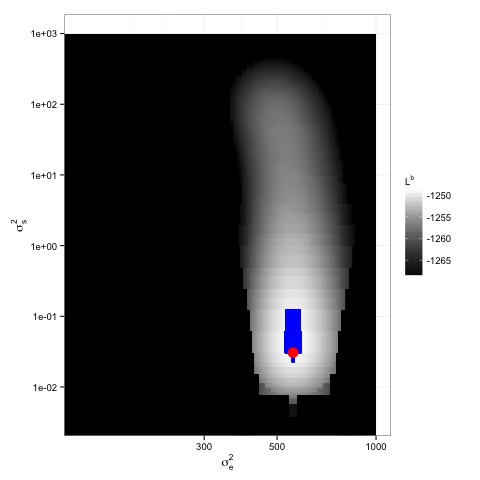
\includegraphics[width=.8\linewidth]{figs/hmo_HH11Bayes_rll.jpg}
	\caption{Grayscale shows $L^b$ in each box.  Red dot shows $b^* \equiv\argmax L^b$.
	Boxes outlined in blue have $U^b \ge L^{b^*}$.  Axes are logarithmic.}
	\label{fig:hmoBayesrll}
  \end{subfigure}
  \caption{The 3,182,803 boxes in the Bayesian analysis of the HMO data.
               $\maxit=20; \epsilon=1; \delta_e=0; \delta_s=0; \text{and\ } M=10$.}
  \label{fig:hmoBayes}
\end{figure}

\subsection{Global Mean Surface Temperature}
We reanalyze a data set in \cite{hodges:2013}, global mean surface temperatures (GMST) from 1881 through 2005, depicted in Figure~\ref{fig:gmst-scatter}.  
\begin{figure}
	\centering
	\includegraphics[width=.5\linewidth]{figs/gmst-scatter.pdf}
	\caption{Global mean surface temperature annually from 1881.
		The $y$-axis shows deviations from the overall mean in units of
		.01 degrees C.}
	\label{fig:gmst-scatter}
\end{figure}
As shown in \cite{ruppert_etal:2003}, many splines can be written as as linear mixed models.  \cite{hodges:2013} fit a piecewise quadratic spline to the GMST data, though a piecewise cubic spline would look similar.  Both splines can be formulated as linear mixed models.  We follow his lead in fitting a quadratic spline with knots at 1880, 1884, 1888, \dots, 2004.  $X$ has three columns: $\textcompute{1}, \textcompute{year}, \textcompute{year}^2$.  $Z$ is $125 \times 30$: one row for each year; one column for each knot.
\begin{equation*}
Z =	\begin{bmatrix}
		0 & 0 & \dots & 0\\
		0 & 0 & \dots & 0\\
		0 & 0 & \dots & 0\\
		0 & 0 & \dots & 0\\
		1 & 0 & \dots & 0\\
		4 & 0 & \dots & 0\\
		9 & 0 & \dots & 0\\
		16 & 0 & \dots & 0\\
		25 & 1 & \dots & 0\\
		\vdots & \vdots & \vdots & \vdots\\
		13924 & 12996 & \dots & 4\\
		14161 & 13225 & \dots & 9\\
		14400 & 13456 & \dots & 16\\
		14641 & 13689 & \dots & 25\\
	\end{bmatrix}; \hspace{.5cm} \Sigma_e = \mathbf{1}_{125}; \hspace{.5cm}
		\Sigma_s = \mathbf{1}_{30}
\end{equation*}
Because we fit a quadratic spline, the entries in $Z$ are squares.  $\Sigma_e$ and $\Sigma_s$ are identity matrices of the appropriate dimension.  See \cite{hodges:2013} for details.  Following Hodges, we center and scale the \textcompute{year} column of X, then compute the $\textcompute{year}^2$ column of $X$ and all the columns of Z from the transformed \textcompute{year}, so Z becomes
\begin{equation*}
Z =	\begin{bmatrix} 
		0 & 0 & \dots & 0\\
		\vdots & \vdots & \vdots & \vdots\\
		10.97143 & 10.2521 & \dots & 0.01219048\\
		11.15505 & 10.42971 & \dots & 0.01904762\\
	\end{bmatrix}
\end{equation*}
Centering and scaling changes only the scale on which $\sigssq$ is measured; we do it to more easily compare our result to Hodges'.

The column space of $Z$ shares no dimensions with the column space of $X$ so $s_z=30$ and, for our $\logRLorig$ analysis, there are 31 lines in all, for $j=1,\dots,31, v$, as shown in Figure~\ref{fig:gmst-lines}.
\begin{figure}
	\centering
	\includegraphics[width=.5\linewidth]{figs/gmst-lines.pdf}
	\caption{The 31 lines, $j=1, \dots, 30, v$, for the $\logRLorig$ analysis of
	              global mean surface temperatures.}
	\label{fig:gmst-lines}
\end{figure}
Our first run of the algorithm used the box determined by the largest intercepts of the 31 lines on the $\sigesq$ and $\sigssq$ axes and the control constants 
\begin{equation*}
	\maxit=15; \hspace{1cm} \epsilon=10; \hspace{1cm}
	\delta_e=1; \hspace{1cm} \delta_s=1; \hspace{1cm} M=10.
\end{equation*}
After 15 iterations there were 3740 boxes still in the active list and 52,973 in the inactive list; they are displayed in Figure~\ref{fig:gmst1}.

\begin{figure}
  \begin{subfigure}{.5\textwidth}
    \centering
    \includegraphics[width=.8\linewidth]{figs/gmst-boxes1.pdf}
    \caption{Locations of boxes}
    \label{fig:gmst-boxes1}
  \end{subfigure}
  \begin{subfigure}{.5\textwidth}
    \centering
    \includegraphics[width=.8\linewidth]{figs/gmst-rll1.pdf}
    \caption{Grayscale shows $L^b$ in each box.
                  Red dot shows $b^* \equiv\argmax L^b$.
	          Boxes outlined in blue have $U^b \ge L^{b^*}$.
	          Axes are logarithmic.}
    \label{fig:gmstrll1}
  \end{subfigure}
  \caption{The 56,713 boxes from the first, coarse, analysis of global
                mean surface temperature.}
\label{fig:gmst1}
\end{figure}

The figure shows that the algorithm needed to divide boxes near the axes more finely than boxes away from the axes and that high $\logRLorig$ is found in only a small region of the plot and therefore suggests rerunning the algorithm with a smaller initial box while imposing more stringent algorithmic parameters.  We limited the starting box to $\sigesq\in(50,500)$, $\sigssq\in(0,10^6)$ and set the control constants to 
\begin{equation*}
	\maxit=20; \hspace{1cm} \epsilon=2; \hspace{1cm}
	\delta_e=0; \hspace{1cm} \delta_s=0; \hspace{1cm} M=10.
\end{equation*}
After 20 iterations there were 1,986,000 active and 1,619,095 inactive boxes.  Results are in Figure~\ref{fig:gmst2}.  The figure agrees with Figure~15.3 in \cite{hodges:2013} and is detailed enough so no further iterations are needed.

\begin{figure}
  \begin{subfigure}{.5\textwidth}
    \centering
    \includegraphics[width=.8\linewidth]{figs/gmst-boxes2.jpg}
    \caption{Locations of boxes}
    \label{fig:gmst-boxes2}
  \end{subfigure}
  \begin{subfigure}{.5\textwidth}
    \centering
    \includegraphics[width=.8\linewidth]{figs/gmst-rll2.jpg}
    \caption{Grayscale shows $L^b$ in each box.
                  Red dot shows $b^* \equiv\argmax L^b$.
	          Boxes outlined in blue have $U^b \ge L^{b^*}$.
	          Axes are logarithmic.}
    \label{fig:gmstrll2}
  \end{subfigure}
  \caption{The 3,605,095 boxes from the second analysis of global
                mean surface temperature.}
\label{fig:gmst2}
\end{figure}

\section{Discussion}
This paper has explained and illustrated an algorithm, for linear mixed models with two variances, to find all regions where either the restricted likelihood function or the joint posterior density of the variances is high, and to evaluate the function there to arbitrary accuracy.  A natural question to ask is \emph{What about linear mixed models with more than two variances?}  A partial answer is given by \cite{hodges:2013} who shows that some models with more than two variances can be reexpressed similarly to \eqref{eq:reexpress} but others can't.  More complex models that can be reexpressed this way include but are probably not limited to models displaying general balance that are also orthogonal designs \citep[all balanced ANOVAs plus other models;][]{houtman_speed:1983}, models that are separable in a specific sense \citep[Section 17.1.5]{hodges:2013}, and miscellaneous other models \citep[Section 17.1.5]{hodges:2013}, e.g., a spatial model including random effects for heterogeneity and spatial clustering (an improper conditional autoregressive effect). We have not explored whether the reexpressible models can be analyzed by our algorithm; that's one direction for future work.  

Another is to see whether the algorithm can be used to advantage even in non-reexpressible models.  If a model has, say, three variances and is now analyzed by, say, MCMC, we can create an MCMC chain that alternates between draws of $(\sigesq,\sigssq)$ and draws of the other variance.  With the aid of our algorithm we may be able to draw more accurately from $[\sigesq,\sigssq\g \sigma^2_\text{other}]$.  More generally, the conditional distribution of $(\sigesq,\sigssq)$ given other parameters can now be analyzed more accurately than in the past.  We have yet to explore how to exploit that accuracy.  A third direction is the posterior $\pi(\sigesq,\sigssq\g y)$.  We can identify a region $B^c$ where the posterior density is low relative to its maximum and it would be of at least mild interest to find an upper bound for the posterior mass of $B^c$.

As written, our algorithm moves a box $b$ to the inactive list if
\begin{enumerate}[(a)]
\item $U^b < L-M$ or
\item $U^b - L^b < \epsilon$ or
\item either the vertical or horizontal extent of $b$ is sufficiently small.
\end{enumerate}
But one could construct more elaborate rules.  One appealing example is to apply criteria (a) and (c) if $U^b \le L-\epsilon_2$ and apply criterion (b) if $U^b > L-\epsilon_2$.  Other rules are possible, too.  We don't elaborate here in order to concentrate on the main ideas.

In this paper we have taken the point of view that it is important to find all regions where $\log f$ is large without necessarily identifying all local maxima or even the global maximum, even though that point of view is at odds with common statistical estimators that maximize the likelihood, the restricted likelihood, or the posterior density.  If two local maxima are close in height it hardly matters which is slightly higher than the other.  And, as we said earlier, if there is a high plateau it hardly matters whether there are little bumps on that plateau.

\bibliographystyle{jasa}
\bibliography{paper}

\end{document}